%Beamer class
\documentclass{beamer}

\usepackage[czech]{babel}
\usepackage[cp1250]{inputenc}
\usepackage{fontenc}
\usepackage{tgheros}
\usepackage{array}
\usepackage{color}
\usepackage{hyperref}

\usetheme{Antibes}
\usecolortheme{crane}


\title[BE1M13VES]{BE1M13VES}
\subtitle[Manufacturing of Electrical Components] {Manufacturing of Electrical Components}
\author[Brejcha]{Michal Brejcha}
\institute[CTU]{CTU in Prague}
\date[Prague, 2017]{Prague, 2017}

\begin{document}
%------------------------------------------------------------------------------
%Uvodni slajd
%------------------------------------------------------------------------------
\frame{\titlepage}

\begin{frame}
\frametitle{Overview} 
\tableofcontents
\end{frame}

\AtBeginSection[]
{
  \begin{frame}
    \frametitle{TOPIC}
    \tableofcontents[currentsection]
  \end{frame}
}

%------------------------------------------------------------------------------
%Capacitance
%------------------------------------------------------------------------------
\section{\texorpdfstring{Capacitance}{Capacitance}}
%------------------------------------------------------------------------------
	\begin{frame}
    \frametitle{Capacitors}
		\begin{tabular}{p{0.3\linewidth} p{0.6\linewidth}}
		\textbf{Parameters:} &
		\begin{itemize}
			\item $C$... capacitance
			\item $\delta$... tolearance
			\item $U$... nominal voltage
			\item $D$... dissipation factor 
			\item $ESR$... equivalent series resistance
			\item $TCC$... temperature coeficient of capacitance
			\item $VCC$... voltage coeficient of capacitance
			\item frequency dependence
		\end{itemize}
		\end{tabular}
  \end{frame}
%------------------------------------------------------------------------------
	%\begin{frame}
    %\frametitle{Design of Varistor}
			%\begin{center}
			%\begin{tabular}{m{0.5\linewidth} m{0.35\linewidth}}
			%\small
			%\begin{itemize}
				%\item shape: typically tablets, pressed from a mixture of polycrystalline semiconductor,
				%\item material: $SiC$ (old), now $ZnO$ with $MnO$, $Sb_2O$, $MgO$, $Bi_2O_3$ and fixed with a glass fibers,
				%\item outlets: burned $AgPd$ pads and soldered $Cu$ wires outlets,
				%\item covering: synthetic or epoxy resin.
			%\end{itemize} & 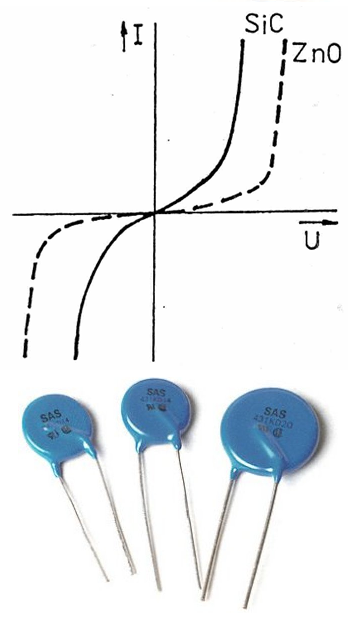
\includegraphics[scale=0.4]{obr15_varPouzdra.png}
		%\end{tabular}
		%\end{center}
  %\end{frame}
%------------------------------------------------------------------------------
\end{document}